%%%%%%%%%%%%%%%%%%%%%%%%%%%%%%%%%%%%%%%%%
% Journal Article
% LaTeX Template
% Version 1.4 (15/5/16)
%
% This template has been downloaded from:
% http://www.LaTeXTemplates.com
%
% Original author:
% Frits Wenneker (http://www.howtotex.com) with extensive modifications by
% Vel (vel@LaTeXTemplates.com)
%
% License:
% CC BY-NC-SA 3.0 (http://creativecommons.org/licenses/by-nc-sa/3.0/)
%
%%%%%%%%%%%%%%%%%%%%%%%%%%%%%%%%%%%%%%%%%

%----------------------------------------------------------------------------------------
%	PACKAGES AND OTHER DOCUMENT CONFIGURATIONS
%----------------------------------------------------------------------------------------

\documentclass[twoside,twocolumn]{article}

\usepackage{blindtext} % Package to generate dummy text throughout this template

\usepackage[sc]{mathpazo} % Use the Palatino font
\usepackage[T1]{fontenc} % Use 8-bit encoding that has 256 glyphs
\linespread{1.05} % Line spacing - Palatino needs more space between lines
\usepackage{microtype} % Slightly tweak font spacing for aesthetics

\usepackage[english]{babel} % Language hyphenation and typographical rules

\usepackage[hmarginratio=1:1,top=32mm,columnsep=20pt]{geometry} % Document margins
\usepackage[hang, small,labelfont=bf,up,textfont=it,up]{caption} % Custom captions under/above floats in tables or figures
\usepackage{booktabs} % Horizontal rules in tables

\usepackage{lettrine} % The lettrine is the first enlarged letter at the beginning of the text

\usepackage{enumitem} % Customized lists
\setlist[itemize]{noitemsep} % Make itemize lists more compact

\usepackage{abstract} % Allows abstract customization
\renewcommand{\abstractnamefont}{\normalfont\bfseries} % Set the "Abstract" text to bold
\renewcommand{\abstracttextfont}{\normalfont\small\itshape} % Set the abstract itself to small italic text

\usepackage{titlesec} % Allows customization of titles
\renewcommand\thesection{\Roman{section}} % Roman numerals for the sections
\renewcommand\thesubsection{\roman{subsection}} % roman numerals for subsections
\titleformat{\section}[block]{\large\scshape\centering}{\thesection.}{1em}{} % Change the look of the section titles
\titleformat{\subsection}[block]{\large}{\thesubsection.}{1em}{} % Change the look of the section titles

\usepackage{fancyhdr} % Headers and footers
\pagestyle{fancy} % All pages have headers and footers
\fancyhead{} % Blank out the default header
\fancyfoot{} % Blank out the default footer
\fancyhead[C]{Running title $\bullet$ May 2016 $\bullet$ Vol. XXI, No. 1} % Custom header text
\fancyfoot[RO,LE]{\thepage} % Custom footer text

\usepackage{titling} % Customizing the title section

\usepackage{hyperref} % For hyperlinks in the PDF

\usepackage{graphicx} %Loading the package

%----------------------------------------------------------------------------------------
%	TITLE SECTION
%----------------------------------------------------------------------------------------

\setlength{\droptitle}{-4\baselineskip} % Move the title up

\pretitle{\begin{center}\Huge\bfseries} % Article title formatting
\posttitle{\end{center}} % Article title closing formatting
\title{Article Title} % Article title
\author{%
\textsc{Frederik Vincent Primdahl} \textsc{Mikael Steenberg Pasovski} \and \textsc{Andreas Peter Brodersen} \textsc{Andreas Wede Gustavsen}\\
\normalsize Copenhagen School of Design and Technology\\ % institution
% \normalsize \href{mailto:john@smith.com}{john@smith.com} % Your email address
%\and % Uncomment if 2 authors are required, duplicate these 4 lines if more
%\textsc{Jane Smith}\thanks{Corresponding author} \\[1ex] % Second author's name
%\normalsize University of Utah \\ % Second author's institution
%\normalsize \href{mailto:jane@smith.com}{jane@smith.com} % Second author's email address
}
\date{\today} % Leave empty to omit a date
\renewcommand{\maketitlehookd}{%
\begin{abstract}
\noindent \blindtext % Dummy abstract text - replace \blindtext with your abstract text
\end{abstract}
}

%----------------------------------------------------------------------------------------

\begin{document}

% Print the title
\maketitle

%----------------------------------------------------------------------------------------
%	ARTICLE CONTENTS
%----------------------------------------------------------------------------------------

\section{Abstract}
In this study the data gathered from customers visiting a hairdresser salon is used to correlate tipping amount with a customer's civil status, age, culture, and the time of day of the visit, to assess which combination of measures affect tipping amount the most. It is proposed that the greatest variance in tipping amount is based on age and civil status, and that these correlate positively with tipping amount, with a married civil status and greater age resulting in higher tips. In addition, this study describes the ethical dilemmas associated with datasets concerning culture. Through analyzation of the dataset, tipping amount is concluded to vary primarily based upon age, with civil status, culture and age as secondary contributing factors.

\lettrine[nindent=0em,lines=3]{L} orem ipsum dolor sit amet, consectetur adipiscing elit.

\section{Ethics} It is important when analysing the data from this study to keep ethics in mind. In this study we deal with data categorized by culture, and therefore a certain bias must be taken into consideration. Maintaining privacy and respecting human rights are just some of the ethical challenges that arise. Keeping ethics into consideration will ensure trust, and accountability to AI that could use the data.
%------------------------------------------------

\section{Methods}
In our analysis we applied the data-driven data science paradigm as to find new insights from the provided haircut tip data set.
As compared to hypothesis-driven data science where a hypothesis/problem is formulated and then data is collected or found to help answer the hypothesis.

This study makes use of the multi-methodological research framework put forth by Nunamaker, and follows four complementary research strategies to alleviate the complexity involved in different research activities. The strategies involve observation, for achieving an understanding of the domain, and to develop hypotheses based on this understanding, theory building in which we examined how to handle the questions from our observation, experimentation, where hypotheses are tested, and finally systems development, for designing and developing the final prototype showcasing the results of the research.

As opposed to a more linear scientific method, the multi-methodological approach supports repeating steps in order to continuously get feedback from previous research activities and gain a more complete understanding of the research area.

For the analyzation of the haircut tipping amount dataset used in this research we make use of inferential statistics, to study a sample group and make generalizations about the wider population. As an extension of this, correlation analysis is also performed to determine how the different variables affect the tipping amount.

Maecenas sed ultricies felis. Sed imperdiet dictum arcu a egestas.
\begin{itemize}
\item Donec dolor arcu, rutrum id molestie in, viverra sed diam
\item Curabitur feugiat
\item turpis sed auctor facilisis
\item arcu eros accumsan lorem, at posuere mi diam sit amet tortor
\item Fusce fermentum, mi sit amet euismod rutrum
\item sem lorem molestie diam, iaculis aliquet sapien tortor non nisi
\item Pellentesque bibendum pretium aliquet
\end{itemize}
\blindtext % Dummy text

Text requiring further explanation\footnote{Example footnote}.

%------------------------------------------------

\section{Analysis}Data cleanup of the initial dataset in this study was needed. First all the undefined columns were removed. Secondly it was needed to format poorly formatted day labels, as these were inconsistent. As an example some were labelled “Tues” and others “Tue”. Converting time to military time was also needed, since the data included a mixed set of 24-hour time and 12-hour time. This ended up in “5” being rewritten as “17”. Lastly we made time and age into integers instead of floats.

To be able to explore and analyse the data, we've chosen to illustrate it using a mix of line and bar diagrams. Figure 1 is the most promising with its clear separation in married and unmarried tip amounts. While figure 1 has been main focus of the study, figure 2 and 3 got shows outliers and are worth exploring.

\begin{figure}[h]
  \centering
  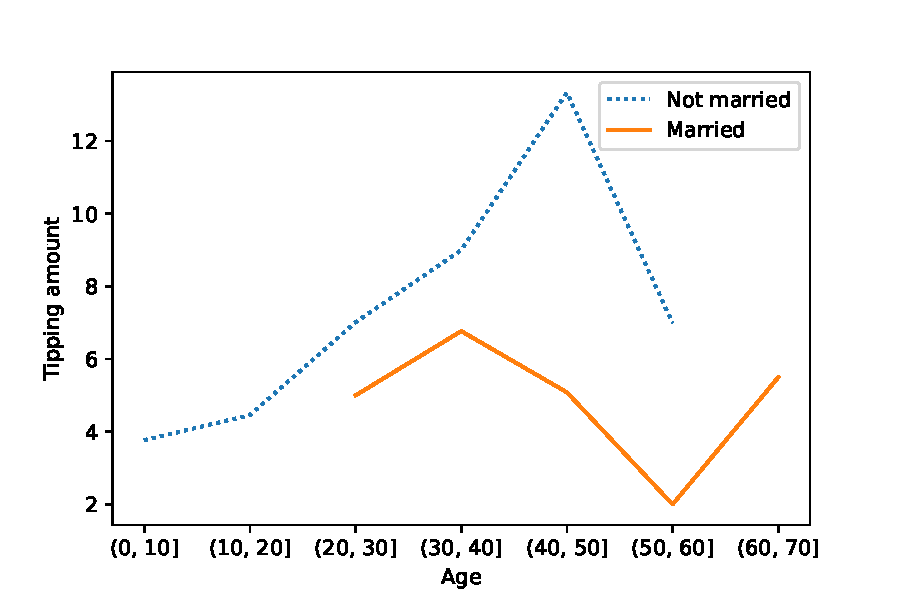
\includegraphics[width=0.5\textwidth]{figures/tip_amount_by_age.pdf}
  \caption{Mean tip amount split by marital status binned by age.}
  \label{fig:tip-amount-by-age}
\end{figure}

\blindtext % Dummy text

\begin{figure}[h]
  \centering
  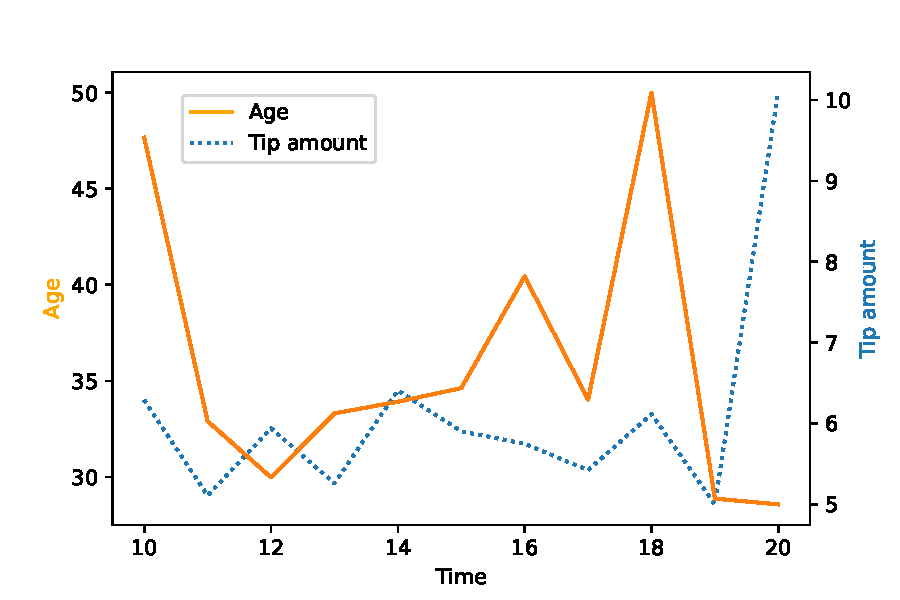
\includegraphics[width=0.5\textwidth]{figures/time_of_day_and_age.pdf}
  \caption{Mean tip amount split by marital status binned by time of day.}
  \label{fig:time-of-day-and-age}
\end{figure}

\blindtext % Dummy text

\begin{figure}[h]
  \centering
  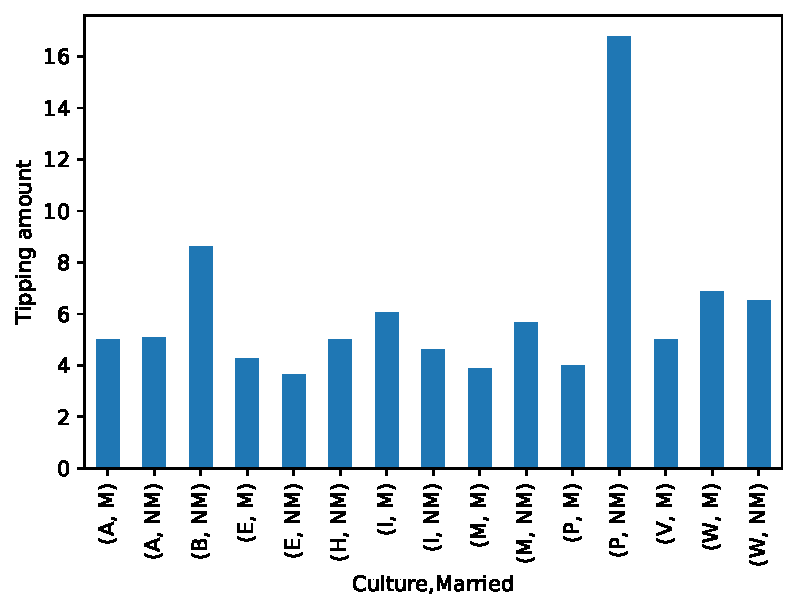
\includegraphics[width=0.5\textwidth]{figures/culture_impact.pdf}
  \caption{Mean tip amount split by marital status binned by culture.}
  \label{fig:culture-impact}
\end{figure}

%------------------------------------------------

\section{Findings}

%------------------------------------------------

\section{Discussion}

\subsection{Subsection One}

A statement requiring citation \cite{Figueredo:2009dg}.
\blindtext % Dummy text

\subsection{Subsection Two}

\blindtext % Dummy text

%----------------------------------------------------------------------------------------
%	REFERENCE LIST
%----------------------------------------------------------------------------------------

\begin{thebibliography}{99} % Bibliography - this is intentionally simple in this template

\bibitem[Figueredo and Wolf, 2009]{Figueredo:2009dg}
Figueredo, A.~J. and Wolf, P. S.~A. (2009).
\newblock Assortative pairing and life history strategy - a cross-cultural
  study.
\newblock {\em Human Nature}, 20:317--330.

\end{thebibliography}

%----------------------------------------------------------------------------------------

\end{document}
